\documentclass[10pt,twoside,notitlepage,a4paper]{report}

\usepackage{verbatim}
\usepackage[hidelinks]{hyperref}
\usepackage{tabularx}
\usepackage{graphicx}
\usepackage{algorithm}
\usepackage{algpseudocode}
\usepackage{cleveref}

\crefname{section}{§}{§§}
\Crefname{section}{§}{§§}

\raggedbottom                           % try to avoid widows and orphans
\sloppy
\clubpenalty1000%
\widowpenalty1000%

\addtolength{\oddsidemargin}{6mm}       % adjust margins
\addtolength{\evensidemargin}{-8mm}

\renewcommand{\baselinestretch}{1.1}    % adjust line spacing to make
% more readable

\setlength{\parskip}{0.5em}%

\newcommand{\python}{\emph{Python}}
\newcommand{\unity}{\emph{Unity}}
\newcommand{\kademlia}{\emph{Kademlia}}
\newcommand{\K}{$k$}

\begin{document}
	
	\bibliographystyle{plain}
	
	\pagestyle{empty}
	
	\hfill{\LARGE \bf Samuel J. Sully}
	
	\vspace*{60mm}
	\begin{center}
		\Huge
		{\bf Voxel Populi:\\ A Decentralised Peer-to-Peer Voxel-Based World} \\
		\vspace*{5mm}
		Computer Science Tripos \\
		\vspace*{5mm}
		Robinson College \\
		\vspace*{5mm}
		2019-20
	\end{center}
	
	\cleardoublepage
	
	\setcounter{page}{1}
	\pagenumbering{roman}
	\pagestyle{plain}
	
	\chapter*{Proforma}
	
	{\large
		\begin{tabular}{ll}
			Name:               & \bf Samuel John Sully\\
			College:            & \bf Robinson College\\
			Project Title:      & \bf Voxel Populi: A Decentralised Peer-to-Peer\\ 
								& \bf Voxel-Based World\\
			Examination:        & \bf Computer Science Tripos -- Part II, July 2020\\
			Word Count:         & \bf \footnotemark[1]\\
			Project Originator: & \bf Samuel John Sully\\
			Supervisor:         & \bf Prof. Jon Crowcroft\\
			Director of Studies:& \bf Prof. Alan Mycroft\\
			Overseers:          & \bf Prof. Marcelo Fiore \& Dr. Amanda Prorok 
		\end{tabular}
	}
	\footnotetext[1]{This word count was computed
		by {\tt command?}
	}
	\stepcounter{footnote}
	
	\section*{Original Aims of the Project}
	My project aimed to create a peer-to-peer 3D world using a distributed hash table (DHT), namely \kademlia{}~\cite{kademlia}. I aimed to explore this decentralised, peer-to-peer approach for Massively Multiplayer Online games (MMOs) to see if such an approach is viable. This was motivated by the advantages of the decentralised approach, such as better load balancing and longevity for the game.
	
	\section*{Work Completed}
	I have completed all the work set out in my proposal, the three parts of my project are all functioning correctly. I implemented \kademlia{} with some modifications to better suit the virtual world application; I implemented the game server to run above the DHT and process the computation for a set of chunks of the world and I implemented the graphical client in \unity{} which connects to the world and allows a user to move around and interact with it. I also completed the test client which was used in the evaluation stage.
	
	\section*{Special Difficulties}
	None.
	
	\newpage
	\section*{Declaration}
	
	I, Samuel John Sully of Robinson College, being a candidate for Part II of the Computer
	Science Tripos, hereby declare that this dissertation and the work described in it are
	my own work, unaided except as may be specified below, and that the dissertation does
	not contain material that has already been used to any substantial extent for a comparable
	purpose.
	
	\bigskip
	
	\noindent I, Samuel John Sully of Robinson College, am content for my dissertation to be made available to the students and staff of the University.
	
	\cleardoublepage
	
	\tableofcontents
	
	\listoffigures
	
	\listoftables
	
	\listofalgorithms
	
	\newpage

	\cleardoublepage
	
	\setcounter{page}{1}
	\pagenumbering{arabic}
	\pagestyle{headings}
	
	\chapter{Introduction}
	
	\section{Project Summary}
	My project explores a peer-to-peer architecture for MMOs or large scale simulations. This is in contrast to the more commonly used centralised approach. My project is build upon a distributed hash table which is used to locate in the peer-to-peer network the server responsible for handling any particular part of the world.
	
	My project consists of three parts: the distributed hash table which is a modified version of the \kademlia{}~\cite{kademlia} specification; the game server which runs the computation for certain segments of the world and the \unity{} client used to interact with the world. All these have been completed in adherence to the success criteria in my project proposal, as well as the evaluation client used in the evaluation stage. The project culminated in a large scale test using Amazon Web Services.
	
	\section{Motivation}
	The Massively Multiplayer Online Game (MMO) genre is very popular\footnote{\emph{World of Warcraft} -- a popular MMO -- had 7.7 million subscribers in 2019.} in modern gaming, as an increasing proportion of the populace have access to high speed broadband the prevalence of these games continues to increase. Most of these games employ a centralised client-server mode where the creators of the MMO have a relatively small number of expensive and powerful machines which they use to handle all players.
	
	This centralised approach often requires some form of `sharding'~\cite{shard}, whereby players are separated into separate, independent instances (`shards') of the same world. Meaning that players can only interact with others connected to the same shard. The centralised approach also means that the game creators have total authoritative control over the game.
	
	An alternative approach is a decentralised, peer-to-peer approach which I explore in this project. In this approach the world is separated into segments (or `chunks') and each peer in the network is responsible for handling the load for a number of chunks. This approach implicitly performs load balancing and is highly failure tolerant, as a node failure can be dealt with by simply having another take over.
	
	This has a number of advantages over the centralised, sharded approach. One significant advantage is that the world is able to be explicitly mutable (such as the voxel-based world I have implemented), with the sharded approach if a player makes a change in one shard then we may need some way of propagating these changes to the other shards while maintaining consistency. However, in my approach there is only one server which is authoritative for the state of any part of the world so there is no need for complex consensus mechanisms.
	
	A further advantage is that the system has improved longevity. When large-scale MMOs cease to be profitable or useful for the developers, who operate the centralised servers, they often shut them down, as recently happened with the popular MMO \emph{Club Penguin}~\cite{clubpenguin} in 2017. With my approach, if we allow individuals to create their own servers to join the peer-to-peer network then, provided there exists a community dedicated to keeping the MMO running, it can continue to exist at no cost to the developers. It would even be possible to have multiple, separate networks running or even networks running modified versions of the game.
	
	\section{Related Works}
	There are very few large-scale, peer-to-peer MMOs, likely due to the security issues I will present in the evaluation chapter and due to the fact that it limits the ability for the developers to monetize the MMO post-release. However, it is possible that techniques similar to mine may be used behind the scenes on a number of large-scale MMOs.
	
	One similar piece of work is \emph{SpatialOS}~\cite{SpatialOS}, this is a platform for managing online games or simulations in the cloud. It works in a similar way to my project, by splitting up the world into segments which are administrated by separate servers. \emph{SpatialOS} is produced by the startup Improbable and is still fairly new, however, it is being used in the development of a number of games.
	
	It's worth noting also that while my implementation of \kademlia{} is custom, I used a \kademlia{} library~\cite{pykademlia} for \python{} as a reference for a fully functioning Kademlia implementation. However, this implementation uses the approach outlined in the second Kademlia paper, while my approach uses the slightly different approach from the first paper.
	
	\cleardoublepage
	\chapter{Preparation}
	
	\section{Starting Point}
	Prior to this project I had limited experience in implementing distributed systems, my knowledge on such systems mainly comes from the Part IB courses Concurrent and Distributed Systems and Computer Networking. Computer Networking introduced the concept of distributed hash tables (DHTs) which are used extensively in my project. Concurrent and Distributed Systems introduces most of the overarching principles of distributed systems, such as RPCs, which are essential in my project. Furthermore, my project relies on knowledge from a number of other courses, such as Part II Principles of Communication and Part IA Introduction to Graphics. I have some limited experience with 3D graphics from my own hobby programming as well.
	
	\section{Requirement Analysis}
	My project aims to implement a suite of software for the operation, interaction with and testing of a 3D world which is distributed over a number of peers in a peer-to-peer network. The success criteria set out in my proposal is as follows:
	
	\begin{enumerate}
		\item My DHT must adhere to the Kademlia specification. It is possible I will need to make some changes to fit the specification better to my needs and this is acceptable.
		\item The peer-to-peer node program must join the network, bootstrapping via some known node, and then will be able to participate in hosting the game world as it becomes part of the DHT.
		\item It must be possible to interact with the world using a simple 3D graphical client, which is able to place and remove voxels from the world. These changes must persist.
		\item The system must handle player moving between separate chunks (and thus, separate peers) seamlessly, with no loading screen.
		\item There must be a simple test agent which connects to and interacts with the world in some notional way to emulate the behaviour of a human user. This is for the purposes of quantitative evaluation.
	\end{enumerate}

	In addition to these criterion, the project will need to fulfil a number of other requirements:
	
	\begin{itemize}
		\item \textbf{Robustness:} the system must be very robust, handling node failures with minimal disruption to the overall system, minimising disruption to users connected to the system at a given time.
		\item \textbf{Deployment:} the implementation must run as a cloud application, being easily deployable to a large number of machines. In my testing I will be using \emph{AWS EC2} Virtual Private Servers running \emph{Ubuntu 18.04}.
		\item \textbf{Decentralisation:} the implementation must be designed to be entirely decentralised, nodes in the P2P network must be entirely equal, there must be no authoritative entity in the system.
		\item \textbf{Mutability:} the game world must emulate that of voxel-based games such as \emph{Minecraft}. As such, users must be able to edit the world and have these changes persist, users' locations must also be stored so that when they log out and back in at another time (or to a different server), they return to where they left off.
	\end{itemize}

	\section{Kademlia}
	My project is built using a DHT at its core, a DHT is a decentralised storage system based on the commonly used hash table data structure. DHTs store \textless key,value\textgreater~pairs, these are distributed among the nodes in the network, with there existing some method to partition the set of keys between the nodes, preferably in such a way that node joins or leaves require minimal changes to this partition (i.e. a node leaving does not cause the entire key-node mapping to change). The DHT maintains an \emph{overlay network} where each node maintains a set of links to other nodes in the DHT according to the topology of the network, this set of links is used in routing queries around the DHT.
	
	\subsection{XOR Metric}
	The \kademlia{} specification sets out that identifiers be $160$bit integers. Nodes IDs and keys for the DHT occupy this ID space. The notion of distance between identifiers, $d(x,y)$, is given by the bitwise XOR of the two (i.e. $d(x,y) = x \oplus y$). This is a valid metric as it obeys the following properties:
	\begin{enumerate}
		\item $d(x,x) = 0$, that is, the distance from any identifier to itself is $0$.
		\item $d(x,y) > 0$ if $x \neq y$, that is, the  distance between any two distinct identifiers is larger than $0$.
		\item $d(x,y) = d(y,x)$, that is, distances are symmetric.
		\item Distances obey  the triangle inequality, i.e. $d(x,z) \leq d(x,y) + d(y,z)$.
	\end{enumerate}
	The set of keys which a node `owns' is given by all those which are closest to its ID using the above notion of distance\footnote{This is not strictly true, actually the \K~closest nodes all store values for that key, where \K~is a parameter of the network.}.
	
	\subsection{Node State}
	Each node maintains some amount of information about other nodes in the network in order to route messages. Each node maintains a \K-bucket for each $i$ in $0 \leq i < 160$ , a \K-bucket is simply a sorted list (of length \K) of \textless IP address, UDP port, node ID\textgreater~triples of nodes between $2^i$ and $2^{i+1}$ distance away from this node. The lists are sorted by time last seen, such that the most recently seen node is at the tail of the list. This is useful later when evicting stale nodes from the \K-bucket. Note that \K~is a parameter of the network, the replication parameter.
	
	In order to populate these \K-buckets, whenever a node receivers a message from another, it looks for the appropriate \K-bucket and, if the sender is already in the \K-bucket then it is moved to the tail of the list, otherwise it is appended to the tail of the list. If the \K-bucket is full then we send a \texttt{PING} RPC to the least recently seen node, if it fails to reply then we evict it and put the new node in instead, else we discard the new node\footnote{In my implementation, the new node is added to a queue to join the \K-bucket.}.
	
	\subsection{RPCs}
	The Kademlia protocol has four RPCs: \texttt{PING}, \texttt{FIND\_NODE}, \texttt{FIND\_VALUE} and \texttt{STORE}. All other operations are built up from these four RPCs. Table \ref{tab:rpcs} details the function of each RPC. My implementation will deviate from this specification as detailed in \cref{sec:customrpc}.
	
	\begin{table}
		\begin{tabularx}{\textwidth}{| l | X |}
			\hline
			\texttt{PING} & Used to check whether a node is online, upon receiving a \texttt{PING} RPC a node will reply with its ID.\\
			\hline
			\texttt{FIND\_NODE} & Takes a $160$bit integer as argument (and identifier). When a node receives a \texttt{FIND\_NODE} RPC it returns \textless IP address, UDP port, node ID\textgreater~ triples from the \K nearest nodes to the argument identifier that it knows of.\\
			\hline
			\texttt{FIND\_VALUE} & Behaves in the same was as \texttt{FIND\_NODE} but will return a value if it possesses one for the supplied ID.\\
			\hline
			\texttt{STORE} & Takes a \textless key, value\textgreater~ pair which the receiving node stores.\\
			\hline
		\end{tabularx}
		\caption{The four \kademlia~RPCs.}
		\label{tab:rpcs}
	\end{table}
	
	\subsection{Node Lookup}
	The lookup procedure is used to locate the \K closest nodes to a supplied identifier. The lookup procedure has one parameter, the concurrency factor $\alpha$. It proceeds as follows:
	\begin{enumerate}
		\item Find $\alpha$ closest nodes from own \K-buckets.
		\item Send \texttt{FIND\_NODE} RPCs to these $\alpha$ nodes searching for supplied identifier.
		\item Then we recursively send \texttt{FIND\_NODE} requests nodes it learned of from the results of previous steps.
		\item When an iteration of RPCs gives us no new nodes better than the current closest, we send RPCs to all of the \K~closest nodes we have not yet queried.
		\item The procedure terminates when we have received a response from all of the \K~nearest nodes.
	\end{enumerate}
	The \K~nearest nodes are returned from this procedure.
	
	\subsection{Value Lookup}
	The procedure for retrieving a value from the DHT is similar to the node lookup procedure above, replacing the \texttt{FIND\_NODE} RPCs in the above description with \texttt{FIND\_VALUE} RPCs. Instead of returning the \K~nearest nodes it will return the value found, or some notional \texttt{NULL} value if none exists.
	
	\subsection{Value Storage}
	The store value procedure consists of performing a lookup node procedure as above with the identifier being the key of the \textless key, value\textgreater~ pair to be stored. Then \texttt{STORE} RPCs with the \textless key, value\textgreater~ pair are sent to the \K~nodes returned from the lookup.
	
	\subsection{Bootstrap}
	Bootstrapping is the process by which a node joins the network. Because \kademlia{} routing information is implicitly learned through network activity we do not need an explicit \texttt{JOIN} method, we can simply use existing RPCs to join a network. All that we need is the IP, port and ID of any existing node in the network, this is the bootstrap node.
	
	The joining node, $n$, inserts the bootstrap node, $m$, into the appropriate \K-bucket and then performs a node lookup for its own ID. Finally it refreshes all its buckets which are further away than its closest neighbour. Refreshing a \K-bucket simple means picking a random ID from that bucket's range and performing a node lookup for that ID. This operation is performed automatically by each node periodically on all buckets which have not been touched in a certain amount of time\footnote{Usually 1 hour.}. By performing a lookup of itself and by refreshing those \K-buckets we have ensured that this node has been inserted into the routing tables of a number of other nodes.
	
	\section{Game Server}
	The second major part of my project is the game server, for this I will use an architecture similar to that used by \emph{Minecraft} and by \emph{Valve}'s \emph{Source} engine~\cite{source}. An instance of a game server will be the authoritative dedicated host that runs the computations for a given set of chunks of the game world, a client will connect to a number of servers in order to receive the current world state and display it to the user graphically. This section of the system is purely client server, clients do not communicate among one another, instead doing so via the server(s).
	
	The server will use an approach used in both \emph{Minecraft} and \emph{Source} where the game world is simulated in discrete time steps known as `ticks'. During a tick we process any incoming packets and update the state of the world, then we send any packets to clients in order to update the world state. In these examples world state is transferred to clients using \emph{delta compression}, where, after the initial sending of the game state, we only send changes that happened since the last tick, this reduces network load.
	
	A number of further approaches could be employed by my implementation, such as compensating for latency and interpolating between ticks. However, these are beyond the scope of my investigation and are thus not a requirement for my project.

	\section{Client}
	The third major part of my project is the client, which will be used to connect to and interact with, the world. This section of the project will require some 3D graphics, thus it will draw on material from the two graphics courses in Part IA and Part IB. I will also need to implement the algorithm for locating and loading the relevant chunks into the world so that the chunks surrounding the player's current location are always loaded.
	
	For this section of the project I decided to use \unity, rather than \emph{LWJGL}, because the graphical element was simpler and as graphics is not the focus of my project this felt appropriate.
	
	\section{World \& Terrain}
	The game world will be analagous to that of \emph{Minecraft}, in that it will consist of voxels (i.e. blocks) arranged in a 3D grid. An example of \emph{Minecraft}'s terrain can be seen in figure \ref{fig:minecraft}. The \emph{Minecraft} world is broken into `chunks' each $16\times16\times256$ blocks, then each chunk is simply a 3D array of block data.
	\begin{figure}
		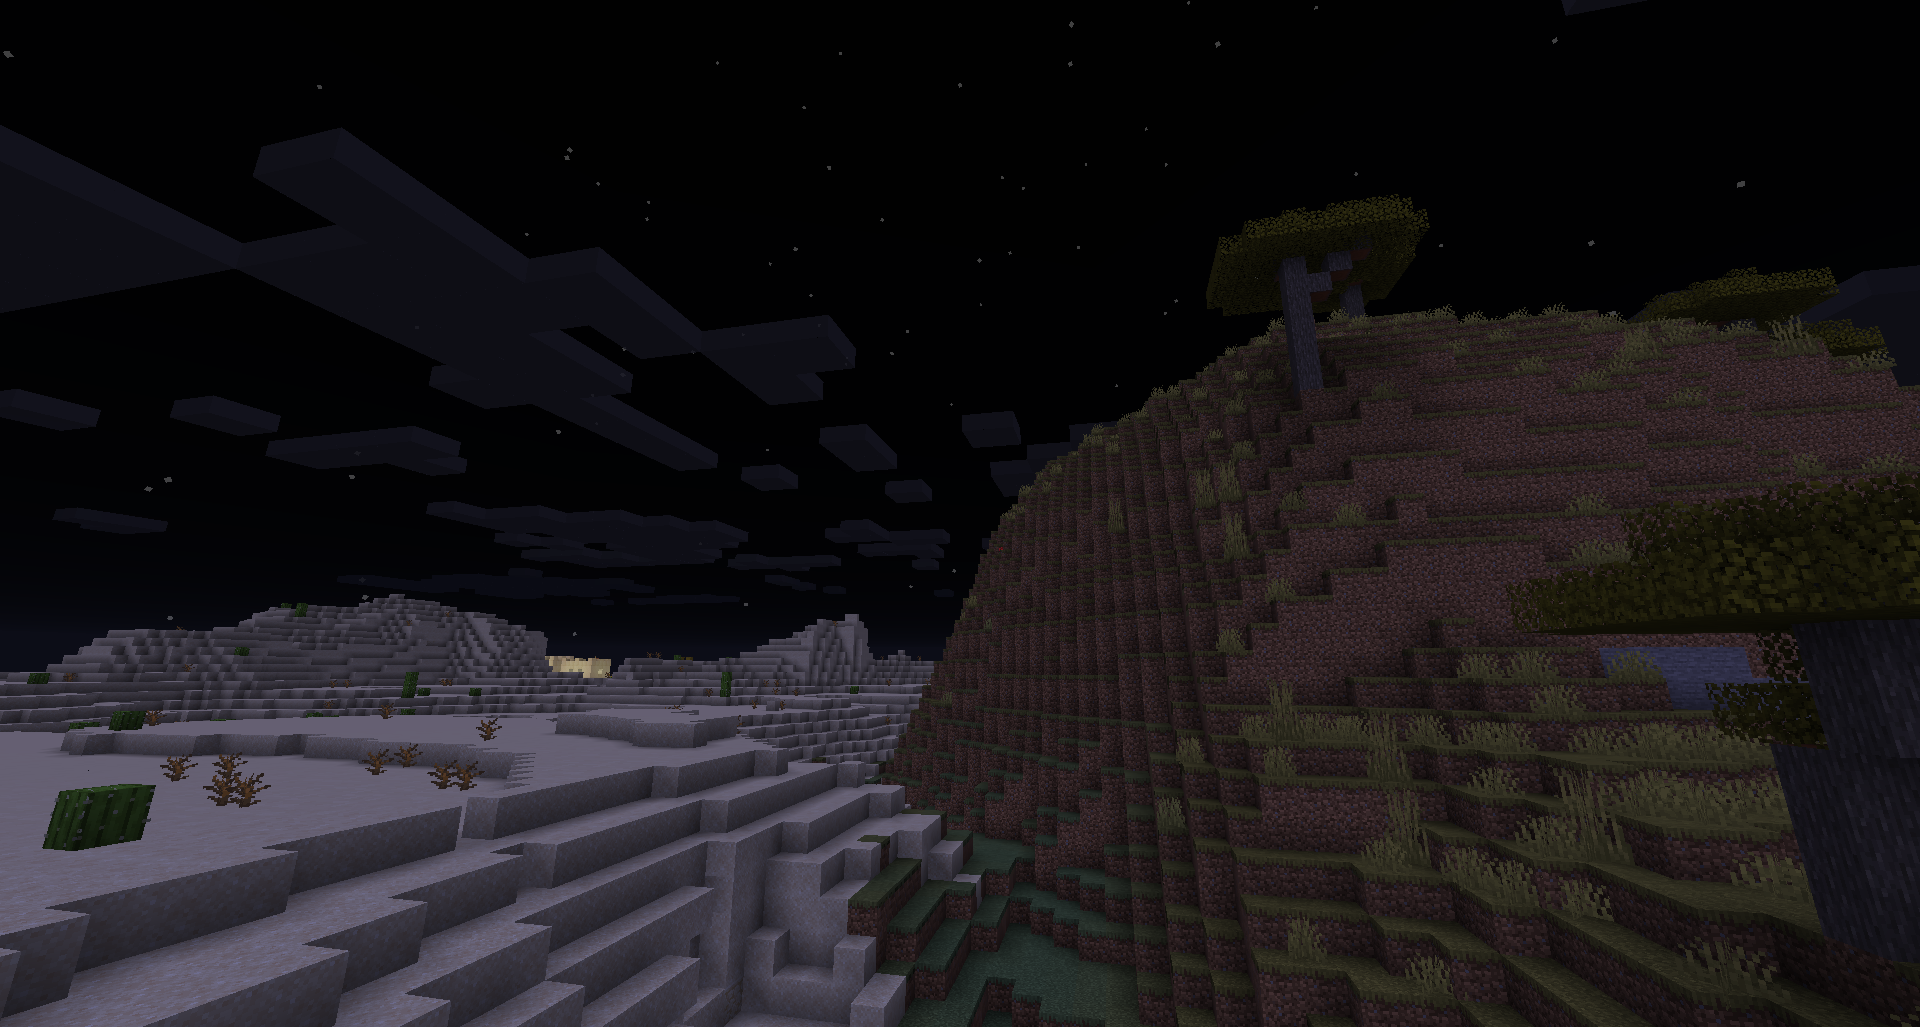
\includegraphics[width=\textwidth]{minecraft.png}
		\caption{A screenshot of terrain from the game \emph{Minecraft}.}
		\label{fig:minecraft}
	\end{figure}

	The terrain in \emph{Minecraft} is generated procedurally, allowing for infinite worlds to be created on the fly. A common approach in procedurally generated video games is to use some form of coherent noise\footnote{Coherent noise simply means smooth pseudorandom noise which obeys the following properties: \begin{enumerate} \item The same input always gives the same output. \item A small change in the input will produce a large change in the output. \item A large change in the input will produce a random change in the output.\end{enumerate}} to generate a height map\footnote{Simply a 2D function or array where the value at any given point is the height of the terrain at any given point.}. I plan to use Perlin noise~\cite{perlin} (or its successor, Simplex noise~\cite{simplex}) to generate a heightmap for my world. Then I will use simple rules to assign blocks at different heights different values (i.e. grass on top, followed by dirt, followed by stone) in order to procude a \emph{Minecraft}-like world. The structure of the world into chunks allows for easy segmentation across servers as each chunk can reside on a different server, additionally, by having data represented within a chunk as a 3D array this makes editing the world simple.
	
	\section{Professional Practice}
	\subsection{Ethical Implications} %pron - persistend customisable environment
	One ethical and legal concern is that my project would give users access to a canvas within which they could, theoretically, encode any data. This could give rise to legal issues if, for example, illegal material were encoded in world data, then the server owner on who's server that data is stored could technically be in breach of the law.
	
	\subsection{Methodology}
	The project was broken up into discrete features, with a timeline planning to complete each in approximately $2-3$ weeks. Thus I followed the \emph{Agile} software development workflow. Each $2-3$ week sprint had a deliverable which could be tested independently and demonstrated. My sprint timetable outlined in the proposal was adapted as the projected moved forward and some parts of the project took more, or less, time than anticipated.
	
	
	\subsection{Tooling}
	I used the \emph{PyCharm} IDE for the development of the \kademlia{} implementation and my game server as these were both written in \python{} using version $3.8$ due to improvements made to the \emph{asyncio} library in \python{} $3.8$. For the client I used \unity{} with \emph{Microsoft Visual Studio 2017} for editing the \emph{C\#} scripts. \emph{Git} was used for version control, with code pushed to \emph{GitHub} regularly and further backed-up daily to both the SRCF\footnote{Student-Run Computing Facility.} and the MCS using a \emph{cron} job.
	
	\subsection{Documentation}
	\textbf{Pending...}	
	
	\cleardoublepage
	\chapter{Implementation}
	My project consists of three parts: the bespoke \kademlia{} implementation, the game server and the client. The system works by having the client query the \kademlia{} implementation to locate the appropriate servers for a particular part of the world, then connecting to that server and `joining' the world via that server. This is visualised in figure \ref{fig:diagram1}.
	
	\begin{figure}
		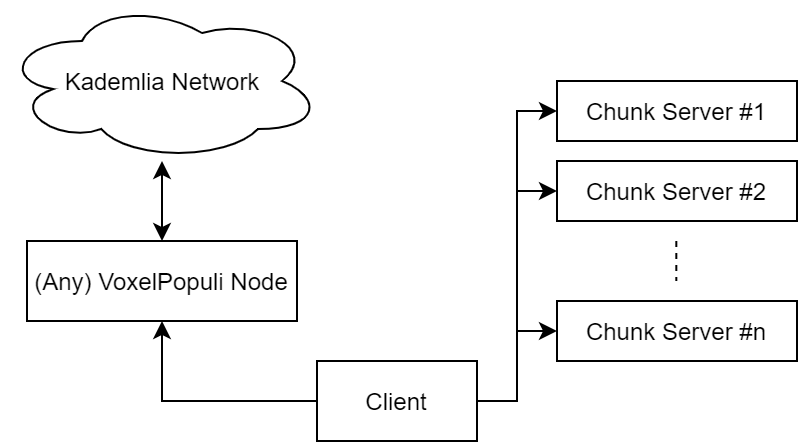
\includegraphics[width=\textwidth]{diag1.png}
		\caption{Diagram giving an overview of \emph{Voxel Populi} architecture. Note that the client needs to know only the IP and port of any node in the Kademlia network, which it will use to access the DHT and query the IP and port pairs of the nodes containing world data it requires.}
		\label{fig:diagram1}
	\end{figure}
	The client needs to connect to a single node from the \emph{VoxelPopuli} network, which it will use as a `stepping stone' to access the whole network via. It uses this stepping stone node to query the DHT to find the \textless IP, port\textgreater~of the game servers responsible for the chunks it needs. It then initiates connections with each of these game servers in parallel, registers the player in that chunk and downloads the world data.
	
	The \emph{VoxelPopuli} server consists of two distinct parts, the \kademlia{} node and the game server. Thus for each node in the network there are two \emph{virtual} nodes. The \kademlia{} nodes are not visible to a client. In order to query the DHT, clients connect to any game server and initiate a special type of session specifically for DHT access. The game server then performs queries to the DHT on behalf of the client. Further details of this special session are in \cref{sec:interface}. Note that for simplicity's sake the \kademlia{} node and game server bind to the same IP address with the game server port being the \kademlia{} port incremented by $1$.
	
	\section{Kademlia}
	This section introduces my bespoke implementation of the \kademlia{} specification. A custom implementation of \kademlia{} was necessary for two main reasons:
	\begin{itemize}
		\item The project necessitated not only \texttt{PUT} and \texttt{GET} procedures but also a \texttt{GENERATE} procedure for locating the appropriate server for a particular chunk and then instructing it to generate said chunk.
		\item Two distinct types of data needed to be stored in the network. The network needed to store chunk location information (IP and port of appropriate server) and player state information in distinct areas so as not to conflate them.
	\end{itemize}
	As such, a custom implementation was devised with additional RPCs and a bespoke high-level interface with the required \texttt{PUT}, \texttt{GET} and \texttt{GENERATE} procedures.
	
	\subsection{Custom RPC Specification}
	\label{sec:customrpc}
	In table \ref{tab:rpcs} I outlined the RPCs in the default \kademlia{} specification. In my implementation I have separate \texttt{STORE\_PLAYER} and \texttt{STORE\_CHUNK} RPCs as well as equivalent variants of the \texttt{FIND\_VALUE} RPCs. These replace the default \texttt{STORE} and \texttt{FIND\_VALUE} RPCs meaning we have a final specification consisting of 6 RPCs: \texttt{PING}, \texttt{FIND\_NODE}, \texttt{STORE\_PLAYER}, \texttt{STORE\_CHUNK}, \texttt{FIND\_PLAYER} and \texttt{FIND\_CHUNK}.
	
	In order to accommodate these new RPCs, the lookup procedure was made polymorphic, taking the appropriate RPC as an argument. Additionally, each node now has two separate storage tables, one for player data and one for chunk data. This implementation was preferable to the alternative of running two distinct \kademlia{} networks, as this would have significant additional overhead as two separate node states would need to be maintained for each node.
	
	\subsection{Generate Procedure}
	When a chunk is found not to exist in the network, it must be generated. In order to do this we need to first locate the server it should be generated on, then we need to check that server is up. Once we have confirmation that the server is running we send a request to the game server on that VoxelPopuli server to generate and initialise the node ready for players. If a node is not up we move to the next nearest node. Once the chunk is generated we must store the \textless IP address, port\textgreater~of the node it was generated on in the network so that in future when we look up this chunk we will find the correct server. Algorithm \ref{alg:generate} gives pseudocode of the generate procedure.
	\begin{algorithm}
		\begin{algorithmic}
			\Function{Generate}{ChunkCoordinate}
				\State $key \gets \mathrm{sha1(ChunkCoordinates)}$
				\State $nodes \gets \mathrm{lookup(key)}$
				\For{$n \in nodes$}
					\State Send generate request to game server at $<n.ip, n.port+1>$ \Comment{Game server address is that of respective \kademlia{} node with port incremented.}
					\If{Successful}
						\State Call RPC \Call{STORE\_CHUNK}{$key, <n.ip, n.port+1>$}
						\State \Return Success
					\EndIf
				\EndFor
				\State \Return Failure
			\EndFunction
		\end{algorithmic}
		\caption{Generate Procedure Pseudocode}
		\label{alg:generate}
	\end{algorithm}
	
	\section{Game Server}
	The game server is responsible for performing the computation and maintaining the state for a number of chunks concurrently. It is also responsible for providing clients with a method of querying the DHT to locate chunks in the \emph{VoxelPopuli} network and to retrieve player data.
	
	\subsection{Server State}
	The game server state consists of a set of active client connections and the state for each of the chunks it is responsible for. Chunk state consists of the world data for that chunk, represented as a 3D array of integers ranging between $0-3$ to represent different voxel types; the set of players currently active in this chunk and their locations; a list of clients who are subscribed to updates on this chunk and $(x,y)$ -- the coordinates of this chunk in the world.
	
	\subsection{Protocol}
	\subsubsection{Handshake Procedure}
	\subsubsection{Game Protocol}
	\subsection{Computation}
	\section{DHT Interface}
	\subsection{Protocol}
	\label{sec:interface}
	\section{Client}
	
	\cleardoublepage
	\chapter{Evaluation}
	
	\cleardoublepage
	\chapter{Conclusion}

	\cleardoublepage
	
	\addcontentsline{toc}{chapter}{Bibliography}
	\begin{thebibliography}{9}
		\bibitem{kademlia} Maymounkov, P. and Mazières, D. Kademlia: A Peer-to-peer Information System Based on the XOR Metric. \url{https://pdos.csail.mit.edu/~petar/papers/maymounkov-kademlia-lncs.pdf}. Accessed: 2019-10-16.
		\bibitem{shard} ``Sharding'' on Wikipedia. \url{https://en.wikipedia.org/wiki/Shard_(database_architecture)}. Accessed: 2019-10-15.
		\bibitem{clubpenguin} ``Club Penguin is shutting down''. \url{https://techcrunch.com/2017/01/31/club-penguin-is-shutting-down/}. Accessed: 2019-10-15.
		\bibitem{SpatialOS} SpatialOS by Improbable. \url{https://improbable.io/spatialos}. Accessed: 2020-03-20.
		\bibitem{pykademlia} Kademlia Python Library. \url{https://github.com/bmuller/kademlia/}. Accessed: 2020-03-20.
		\bibitem{source} Source Engine Multiplayer Networking, Valve. \url{https://developer.valvesoftware.com/wiki/Source_Multiplayer_Networking}. Accessed: 25-3-2020.
		\bibitem{perlin} ``Perlin Noise'' on Wikipedia. \url{https://en.wikipedia.org/wiki/Perlin_noise}. Accessed: 2019-10-17.
		\bibitem{simplex} ``Simplex Noise'' on Wikipedia.
		\url{https://en.wikipedia.org/wiki/Simplex_noise}. Accessed: 2019-03-27.
	\end{thebibliography}
	\cleardoublepage
	
	\appendix
	
	\chapter{Proposal}
	
\end{document}